\section{Setup}
\subsection{General Requirements}
\subsubsection{Hardware requirements}
The only hardware required is to own a CPU newer than a Pentium 4 with SSE2 instruction set.
\subsubsection{Software requirments}
This application can run on GNU/Linux on any distribution newer than Ubuntu 14.04, MacOs from 10.10 onward and Windows from 7 and onward;
Other than an operative system this application needs:
\begin{enumerate}
	\item \textbf{git}: a working version of git cli installed;
    \item \textbf{Node.js}: version 10.16.3 (or higher) need to be installed on your system. To install it, the user can refer to the official web page nodejs.org for installation we recommend the LTS version;
    \item \textbf{npm}: Node Package Manager (npm) version 6.9.0 (or higher) is the package manager that comes with Node.Js;
    \item \textbf{TypeScript}: install the npm package TypeScriptG globally, minimum version required is the 3.6.5;\\\\ \centerline{\code{npm install typescript -g}}\\
    \item \textbf{ts-node}: install the ts-node package globally, minimum version required is the 8.6.0; \newline\newline \centerline{\code{npm install ts-node -g}}\\
\end{enumerate}
For ease of use, the user can also install multiple packages in a single command.
\begin{center}
    \code{npm install typescript ts-node -g}
\end{center}
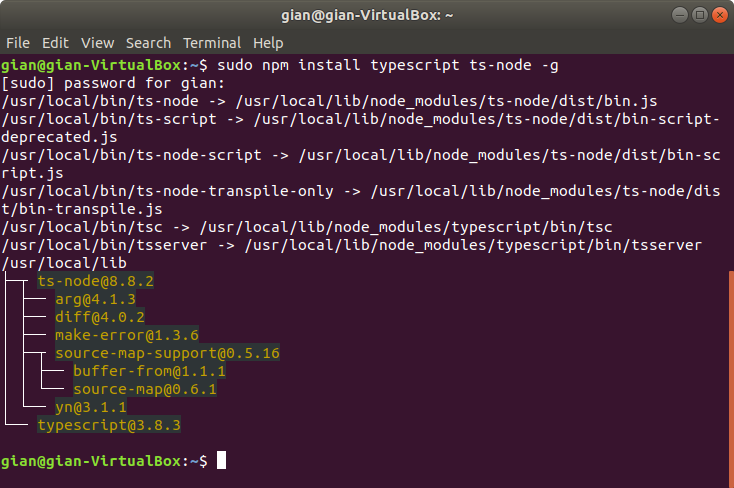
\includegraphics[width=\textwidth]{res/img/typescriptInstall.png}    
Expected procedure outlook.
\subsection{Software download}
A copy of each Etherless component can be retrieved by cloning our github.com repos. For a complete setup, proceed with the following instructions:
\begin{enumerate}
	\item Clone repository \\\\\centerline{\code{git clone https://github.com/TennersUnipd/<componentName>.git}}\\
	\item Move working directory to downloaded folder \\\\\centerline{\code{cd <componentName>-master}}\\
	\item Install all missing dependencies \\\\\centerline{\code{npm install}}\\
\end{enumerate}
Available component names are:
\begin{itemize}
	\item etherless-cli;
	\item etherless-smart;
	\item etherless-server;
\end{itemize}
\subsection{Etherless-cli}
\subsubsection{Requirements}
To develop or run unit tests, \textbf{mocha} needs to be installed
\begin{center}
    \code{npm install mocha -g}
\end{center}
This command will install mocha functionality globally.

\subsubsection{Testing}
Unit test can be run to check if setup has been performed properly:
\begin{center}
    \code{npm run test}
\end{center}

If all tests pass than everything is ready the terminal window will look like the following:
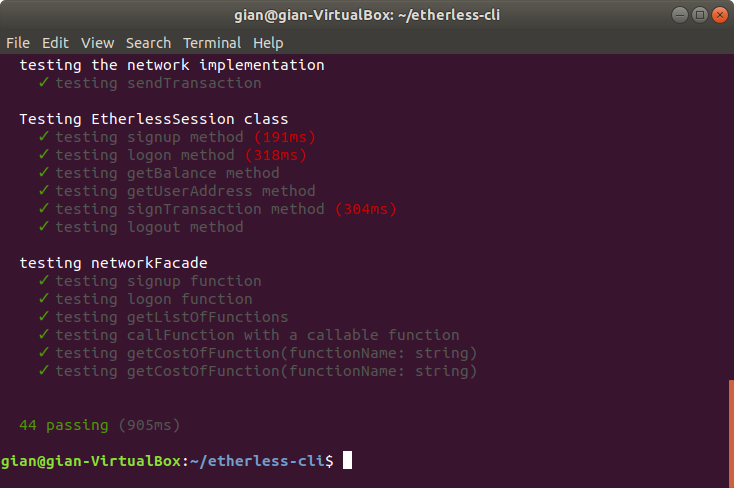
\includegraphics[width=\textwidth]{res/img/npmruntest.png}
Before using the software, the user needs to register to the Ethereum\glo network or log in with an existing private-key\glo, after that, the user needs to add funds to the wallet that can be done through MetaMask\glo importing the account.
\subsubsection{Usage}
To run this program from the command line interface positioning on the main program folder
and type ts-node src/index.ts <<command>> where <<command>> is the command that the user wants to run.\\
\textbf{Attention!} User manual contains a more in-depth explanation of etherless-cli.
\subsubsection{Environments}
The following components are provided for this component:
\begin{itemize}
	\item \textbf{development}: uses local Ethereum\glo network and it's activated by attaching the --dev command option;
	\item \textbf{production}: by default and it uses Ropsten\glo test network;
\end{itemize}
Environment configuration files are \textbf{./.env} and \textbf{./.env.production}.
\\Each configuration specifies the following paramters:
\begin{itemize}
	\item \textbf{PROVIDER API}: connection string to the Ethereum\glo network;
	\item \textbf{ABI PATH}: a path to the contract abi; this file is automatically updated through Etherscan when a new contract address is used;
	\item \textbf{CONTRACT ADDRESS}: deployed smart contract address;
	\item \textbf{ETHSCAN}: an API key for accessing Etherscan service;
	\item \textbf{AWS ENDPOINT}: base endpoint for calling serverless functions;
\end{itemize}
If a configuration parameter is not found in a specialization environment (eg .env.production), its base value will be used from .env.
\subsection{Etherless-smart}
\subsubsection{Requirements}
To run correctly this component the user needs to perform additional installations:
\begin{itemize}
    \item \textbf{Truffle}: to install Truffle please refer to the framework website; \\\\\centerline{\code{npm install Truffle -g}}\\
    \item \textbf{Ganache-cli}: to install ganache cli, please refer to the Truffle framework website;  \\\\\centerline{\code{npm install ganache-cli -g}}
\end{itemize}

\subsubsection{Setup}
\paragraph{Deploy on a local network}
\\Before the deploy on a local network starts, the ganache server needs to be started on a separate terminal instance \code{ganache-cli}
\begin{itemize}
    \item \code{npm install -{}-dotenv-extended} : installs the package with all its dependencies;    
    \item \code{truffle build}: compiles the contracts;
    \item \code{truffle deploy -{}-network local}: deploys compiled contracts to local network (default connection parameters are used);
    \item \code{truffle test}: run contract tests.
\end{itemize}
\textbf{Note!} Ganache can be used with a GUI too.\\\\
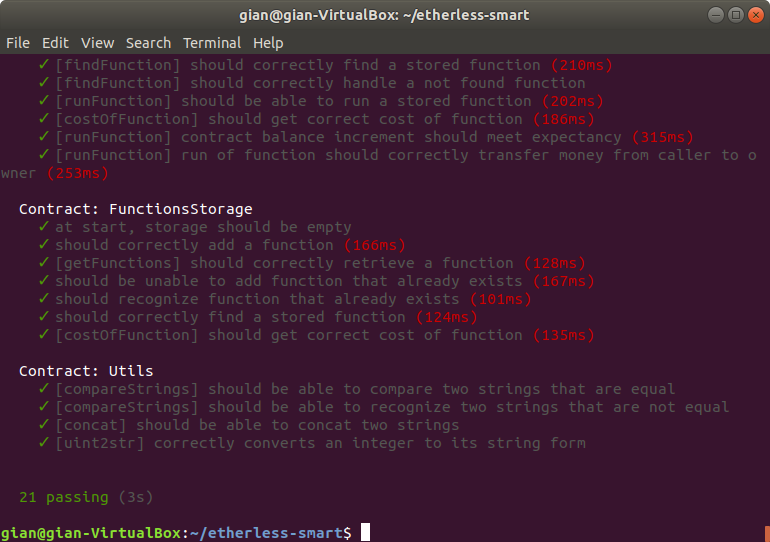
\includegraphics[width=\textwidth]{res/img/truffleTest.png}
Tests execution results.
\paragraph{Deploy on a production like envoirment}
Before the deploy on a production-like network the user needs three different keys: an Etherscan API
key, and Infura account and na Ethereum\glo account with some funds.\\
After obtaining the credentials the user needs to edit the truffle-config.js file replacing all necessary fields. \\
Etherless-smart can be run in a production-like environment
by running the following commands from the component folder:
\begin{itemize}
    \item \code{npm install -{}-dotenv-extended} : installs the package with all its dependencies;
    \item \code{truffle build}: builds the smart contract to obtain the ABI file that is the Smart Contract representation;
    \item \code{truffle deploy -{}-network test}: deploys the compiled smart contract to the Ropsten test network;
    \item \code{truffle run verify EtherlessSmart -{}-network test}: validates the contract on Etherscan; this step is needed for Etherscan to confirm the source code of the application and make available for a download the contract ABI; other components will use this service to update their ABIs\glo
\end{itemize}
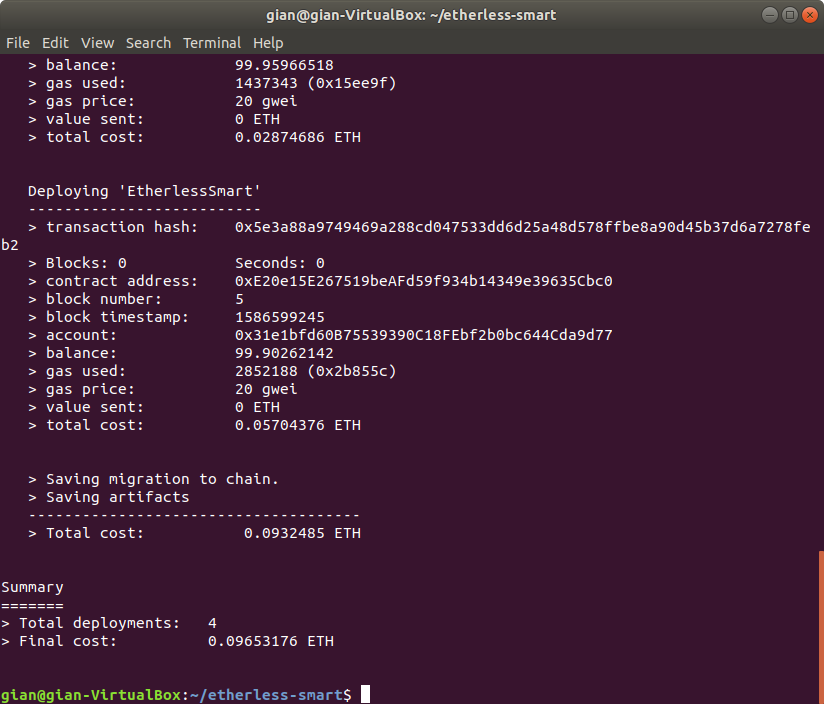
\includegraphics[width=\textwidth]{res/img/deployContract.png}
After the deploy is a good practice to save the contract address somewhere safe as that will be needed to retrieve the contract later.
\subsubsection{Usage}
After the deploy, the contract will be accessible through the network at its assigned address;
\subsubsection{Environments}
The following components are provided for this component:
\begin{itemize}
	\item \textbf{local}: contracts are deployed on a local network;
	\item \textbf{test}: contracts are deployed on the Ropsten\glo test network;
\end{itemize}
Each environment might be caracterized by different configuration parameters and they depend on the connection provider. Configurations can be found in the \textbf{truffle-config.js} file.
\subsubsection{Infura}
Infura is a service that provides access to Etherem networks through their owned network nodes.
\subsection{Etherless-Server}
\subsubsection{Requirements}
The following are required for correctly using and deploying etherless-server:
\begin{itemize}
	\item \textbf{AWS account}: a AWS account is needed to use Lambda and Elastic Beanstalk;
	\item \textbf{Serverless.com account}: an account is needed to use their framework;
\end{itemize}
\subsubsection{Setup}
This component runs on two AWS services Elastic Beanstalk and Lambda.
To be able to run and deploy etherless-server, the following steps are necessary for a proper configuration:
\begin{enumerate}
	\item Setup you AWS credentials (either through the .aws/credentials file or with aws cli);
	\item \textbf{serverless}: to install serverless\glo the user needs to run \code{npm install serverless -g}; this operation will install globally the commands serverless and sls;
	\item Configure serverless AWS credentials using the command\\\\\centerline{\code{serverless config credentials --provider aws --key <key> --secret <secret>}}\\
    \item \textbf{mocha}: to install mocha the user needs to run \code{npm install mocha -g}, this operation will install globally the command mocha which is used for testing;
    \item \textbf{eb}: to install eb cli please refer to the AWS Elastic Beanstalk documentation;
    \item Configure eb by following the instrictions provided by: \\\\\centerline{\code{eb init -i}}\\

\end{enumerate}
\subsubsection{Serverless Functions deployment}\\
To deploy an updated version of the serverless\glo functions, run the command:
\\\\ \centerline{\code{sls delpoy}}
\subsubsection{Serverless Runner deployment}
The runner component runs on the Elastic Beanstalk Amazon's service. To deploy the application correctly the user has to complete the following steps:
\begin{enumerate}
	\item Compile TypeScript\glo to JavaScript\glo \\\\ \centerline{\code{tsc}}
	\item Deploy the codebase \\\\ \centerline{\code{eb deploy <envName>}}
\end{enumerate}
\subsubsection{Local Runner}
For development purposes, a local instance of the runner can be started with the following command:\\\\\centerline{\code{ts-node local.ts}}
\begin{enumerate}
	\item Compile TypeScript\glo to JavaScript\glo \\ \centerline{\code{tsc}}
	\item Select deployment environment \\ \centerline{\code{eb use <envName>}}
	\item Deploy the codebase \\ \centerline{\code{eb deploy}}
\end{enumerate}
\subsubsection{Environments}
\paragraph{Runner}
The runner can be deployed at different stages by making use of eb environments. An environment is an independent instance of the Runner and it connects to a given contract.
\begin{itemize}
	\item To create a new environment use:\\ \centerline{\code{eb create <envName>}}
	\item To select an environment use:\\ \centerline{\code{eb use <envName>}}
\end{itemize}
\paragraph{Serverless Functions}
AWS Lambda supports deployments for different environments. Environment can be set inside the \textbf{serverless.yml} file.